\documentclass{article}
%\usepackage[a4paper, margin=1in]{geometry}
\usepackage{datetime}
\usepackage{wrapfig}
\usepackage[pdftex]{graphicx} \pdfcompresslevel=9
\usepackage[T1]{fontenc}
\usepackage{lmodern}

\usepackage[a4paper, left=2cm,
            right=2cm,
            top=1cm,
            bottom=1.5cm,
            footskip=.5cm]{geometry}
\newdate{date}{26}{01}{2025}
\date{\displaydate{date}}


\title{Introduction au Graphisme: projet personnel}
\author{Camille Schreck}

\begin{document}

\maketitle


\begin{figure*}[h]
  \centering
  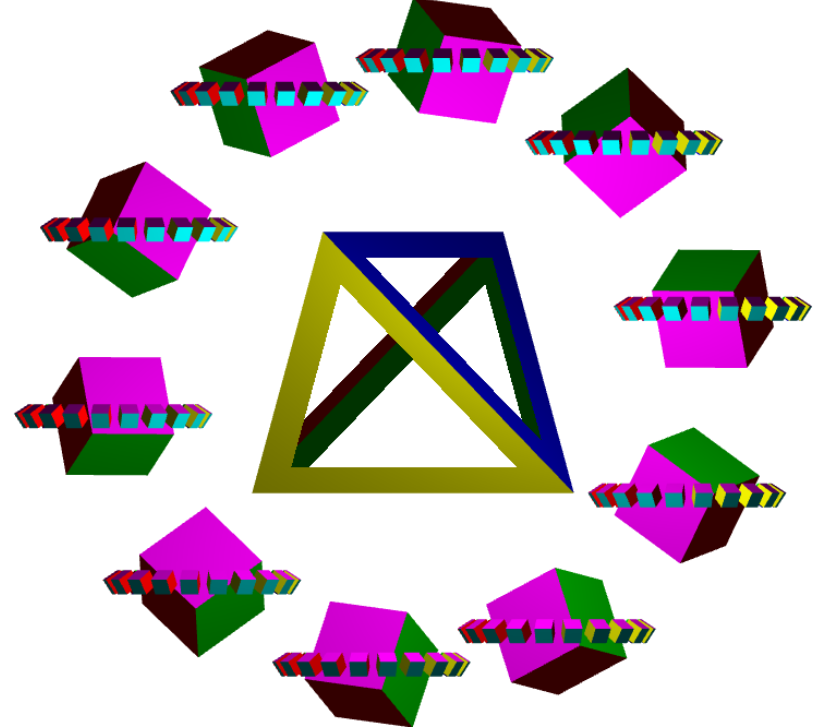
\includegraphics[width=0.6\linewidth]{tet_and_cubes}
\end{figure*}


\section*{Exercice 1: Cubes en orbite}

\begin{enumerate}
\item Cr\'eer un cercle de \texttt{n} cubes tournant autour du centre de la sc\`ene  dans le plan \texttt{(xy)}.
\item Faire orbiter \texttt{m} petits cubes autour des \texttt{n} premiers dans le plan \texttt{(xz)}.
\item Faire tourner les cubes \'egalement sur eux-m\^emes.
\end{enumerate}

\begin{figure*}[h]
  \centering
  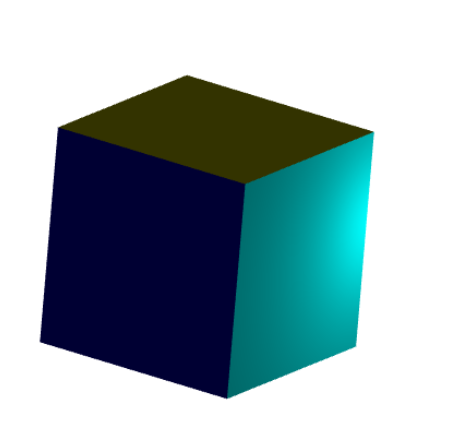
\includegraphics[width=0.3\linewidth]{cube}
  \hspace{1cm}
  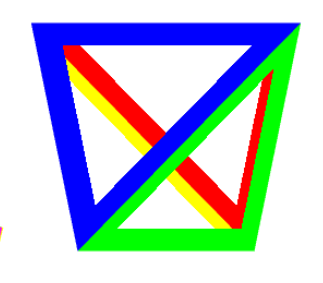
\includegraphics[width=0.3\linewidth]{tet}
\end{figure*}


\section*{Exercice 2: Cube et lumi\`ere}
\begin{enumerate}
\item Cr\'eer un cube au centre de la sc\`ene qui tourne sur lui-m\^eme.
\item Cr\'eer un attribut \emph{normal}, contenant les normales à la surface du cube pointant vers l'extérieur pour chaque vertex du cube.
\item Dans le vertex shader, transformer les normales de sorte qu'elles soient orient\'ees correctement.
  Attention: les normales doivent rester des vecteurs unitaires.
\item \'Etant donn\'ee une source de lumi\`ere situ\'ee en \texttt{(1, 0, 0)}, utiliser ces normales dans le fragment shader pour \'eclairer de fa\c con diffuse les cubes.
\item Faire tourner la lumi\`ere autour du cube.
\end{enumerate}


\section*{Exercice 3: T\'etra\`edre}

\begin{enumerate}
\item Afficher un t\'etra\`edre quelconque au centre de la sc\`ene qui tourne sur lui-m\^eme.
\item \'Evider l'int\'erieur des faces du t\'etra\`edres \`a l'aide de la commande \texttt{discard}. Pour cela, vous pouvez cr\'eer un nouvel attribut représentant les coordonn\'ees barycentriques à l'intérieur de chacune des faces. 
\end{enumerate}

\begin{figure*}[h]
  \centering
  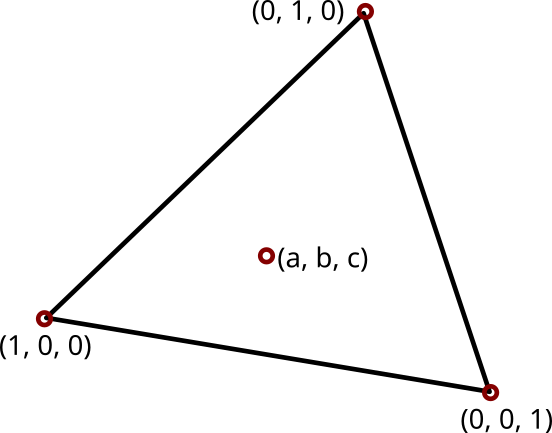
\includegraphics[width=0.3\linewidth]{barycentres}
\end{figure*}

\section{Question bonus}

Combiner les 3 exercices dans une m\^eme sc\`ene.

\end{document}

